Dadas las incoherencias encontradas en los resultados de la sección anterior, se aplica QAOA al problema descrito en el artículo \cite{solving_shortest_path_with_qaoa}, con el fin de seguir analizando el comportamiento del algoritmo al aumentar el número de capas.

Este problema consiste, de nuevo, en obtener el camino más corto para un grafo, en este caso el de la \textit{figura \ref{fig:zhiqiang grafo}}.

\begin{figure}[htbp]{fig:zhiqiang grafo}{Basado en el \textit{artículo \cite{solving_shortest_path_with_qaoa}}}
  \centering
  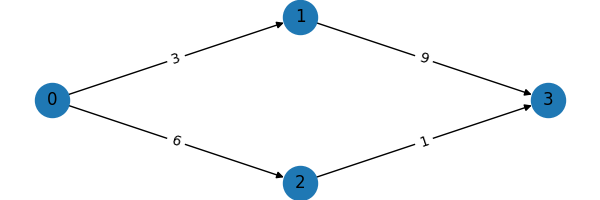
\includegraphics[scale=0.75]{zhiqiang-grafo/zhiqiang-grafo}
\end{figure}

\subsection{Resultados de Qiskit}
\begin{table}[htbp]{tab:5-zhiqiang-aer_estadisticas}{Resultados de la ejecución de QAOA del tercer grafo. P=20. Modificadores del paper (omitir \(2*\gamma\))}
  \centering
  \begin{tabular}{|c|r|r|}
    \hline
    \textbf{nº Capas} & \textbf{Estadística máxima (\%)} & \textbf{Estadística global (\%)} \\ \hline
    p = 1 &  0.6\% &  5.9\% \\ \hline
    p = 2 & 30.7\% & 16.9\% \\ \hline
    p = 3 & 93.8\% & 26.0\% \\ \hline
    p = 4 & 66.9\% & 39.4\% \\ \hline  % EL OTRO MAX RESULTADO OBTENIDO (0101 - 33.1%) ES EL SEGUNDO VALIDO, ESO ES POCO COMÚM
    p = 5 &  1.6\% & 15.0\% \\ \hline  % EL OTRO MAX RESULTADO OBTENIDO (0101 - 98.4%) ES EL SEGUNDO VALIDO, ESO ES POCO COMÚM. El global resultado es 0101 con un 55.17%
    p = 6 & 81.0\% & 32.9\% \\ \hline
    p = 7 & 36.5\% & 26.4\% \\ \hline
    p = 8 & 64.2\% & 32.8\% \\ \hline
  \end{tabular}
\end{table}

A diferencia de las ejecuciones del primer grafo (\textit{tabla \ref{tab:5-primer-paper-aer_estadisticas}}), aquí se ve una clara mejora con el aumento del número de capas.

Además, para el caso \(p = 3\) se aprecia una distancia mucho mayor a la habitual entre la estadística máxima y global. A efectos prácticos se toma como medida de fiabilidad la estadística máxima, ya que significa que se ha encontrado el camino óptimo el 93.8\% de las ejecuciones realizadas.

El resultado de la función gamma es el siguiente:
\begin{figure}[htbp]{}{Función gamma del tercer grafo. P=20}
  \centering
  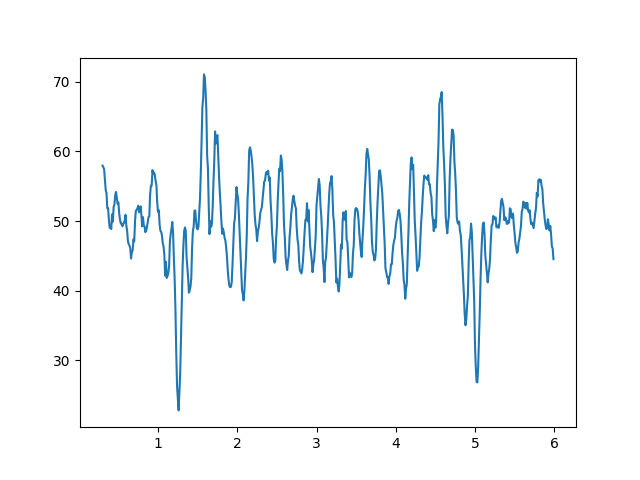
\includegraphics[scale=0.5]{zhiqiang-grafo/modificadores-paper/zhiqiang-p20-gammaFun}
\end{figure}
A diferencia de las funciones gamma del grafo para el problema de MAX-CUT y el primer grafo de QAOA, en esta gráfica se ve mucho más ruido.

Esto se compara también con la gráfica resultante de ejecutar este mismo problema utilizando, para los operadores lineales del circuito, los ángulos obtenidos teóricamente (en lugar de basarse en los obtenidos del artículo).

\begin{table}[htbp]{}{Resultados de la ejecución de QAOA del tercer grafo. Ángulos teóricos}
  \centering
  \begin{tabular}{|c|r|r|}
    \hline
    \textbf{nº Capas} & \textbf{Estadística máxima (\%)} & \textbf{Estadística global (\%)} \\ \hline
    p = 1 &  0.1\% &  9.79\% \\ \hline
    p = 2 & 10.0\% & 20.20\% \\ \hline
    p = 3 & 38.1\% & 19.47\% \\ \hline
    p = 4 &  0.7\% & 27.33\% \\ \hline  % el 99.3\% de resultados ha sido 0101 (en lugar de 1010)
    p = 5 & 40.6\% & 24.29\% \\ \hline
    p = 6 & 30.7\% & 29.29\% \\ \hline
    p = 7 & 49.3\% & 24.60\% \\ \hline
    p = 8 & 71.4\% & 36.34\% \\ \hline
  \end{tabular}
\end{table}

% FIXMEEEEEE: Tal vez quitar? No es significativo. Si se queda comentar la tabla.
\begin{table}[htbp]{}{Resultados de la ejecución de QAOA del tercer grafo. P=40}
  \centering
  \begin{tabular}{|c|r|r|}
    \hline
    \textbf{nº Capas} & \textbf{Estadística máxima (\%)} & \textbf{Estadística global (\%)} \\ \hline
    p = 1 &    0\% &  7.43\% \\ \hline
    p = 2 & 40.3\% & 14.69\% \\ \hline
    p = 3 & 62.0\% &  21.9\% \\ \hline
  \end{tabular}
\end{table}

\subsection{Resultados de D-Wave}
\begin{table}[htbp]{}{Resultados de la ejecución del tercer grafo en D-Wave}
  \centering
  \begin{tabular}{|c|r|r|}
    \hline
    \textbf{Camino} & \textbf{Energía} & \textbf{Número de ocurrencias} \\ \hline
    1010 (\textbf{Óptimo}) &  7 & 776 \\ \hline
    0101                   & 12 & 247 \\ \hline
    0010                   & 46 &   1 \\ \hline
  \end{tabular}
\end{table}

Al igual que en anteriores ejecuciones utilizando Quantum Annealing, se mantiene la coherencia en los resultados. El resultado obtenido un mayor número de veces es el camino óptimo y el siguiente camino más producido es el otro único camino válido (sin romper ninguna restricción).

%%% Local Variables:
%%% mode: latex
%%% TeX-master: "../tfgtfmthesisuam"
%%% End:
